\section{Results}
\subsection{The two-state gap is real but not self-explanatory}
The original confirmation stopped at $N=40$. GPT-5.5 showed positive prompt-level mean-score \live{}--\post{} association ($\rho=.599$, one-sided $p=.00147$ against $\rho_0=.2$). Gemini's mean $P-L$ shift was $+22.83$ points ($p=6.9\times10^{-7}$), exceeding GPT-5.5's shift by $19.02$ points ($p=.00111$). Thus an online score can retain information about a model's later judgment while changing substantially in level. But this two-state result does not identify why it changes.

\subsection{IKEA-like writer-state bias is uncommon}
Table~\ref{tab:decomp} reports the six-model decomposition. Gemini is the only model with a positive mean $R-L$: $+2.77$ points on 40 prompts. The other five means are negative, from $-3.01$ to $-8.40$. In this probe, systematic self-favoring on the original writing trajectory is therefore not the dominant cross-model pattern.

\begin{table}[t]
\centering
\caption{Three-state decomposition. $R-L>0$ is IKEA-like; $P-R>0$ is the Gogol direction. The four breadth-extension sample sizes are adaptive.}
\label{tab:decomp}
\small
\begin{tabular}{lrrr}
\toprule
Model & $N$ & $R-L$ & $P-R$\\
\midrule
GPT-5.5 & 40 & $-3.10$ & $+6.91$\\
Gemini 3.1 Pro & 40 & $+2.77$ & $+20.06$\\
GPT-OSS-120B & 8 & $-6.48$ & $+10.00$\\
DeepSeek V4 Flash & 12 & $-8.40$ & $+3.18$\\
Llama 3.3 70B & 24 & $-3.81$ & $+0.24$\\
Claude Opus 5 & 24 & $-3.01$ & $-2.05$\\
\bottomrule
\end{tabular}
\end{table}

This result does not contradict prior ownership/self-attribution studies: REPLAY is not a direct ownership manipulation. It only shows that the transition from the native writing trajectory to our reconstructed prefix rarely moves in the IKEA-like direction.

\subsection{Post-completion self-devaluation is more frequent and larger}
$P-R$ shows a different pattern. GPT-5.5 and Gemini shift by $+6.91$ and $+20.06$ points on the fixed 40-prompt set ($p=7.8\times10^{-14}$ and $5.8\times10^{-11}$, one-sided tests). For Gemini, $20.06/22.83\approx88\%$ of the total \live{}--\post{} change appears only after completion.

The breadth extension adds two positive cases. GPT-OSS-120B reaches a mean $P-R=+10.00$ at total $N=8$; the four fresh extension prompts cross the sequential correction ($p_{\rm adj}=.021$). DeepSeek V4 Flash reaches $+3.18$ at $N=12$ with fresh-extension $p_{\rm adj}=.040$. Llama remains near zero at the 24-prompt cap ($+0.24$), and Claude moves oppositely ($-2.05$). We therefore do not claim universality. The empirical statement is narrower: positive completion-associated self-devaluation appears in four of six decomposed models and dominates the strongest observed shifts, whereas a positive IKEA-like mean appears in one.

\begin{figure}[t]
\centering
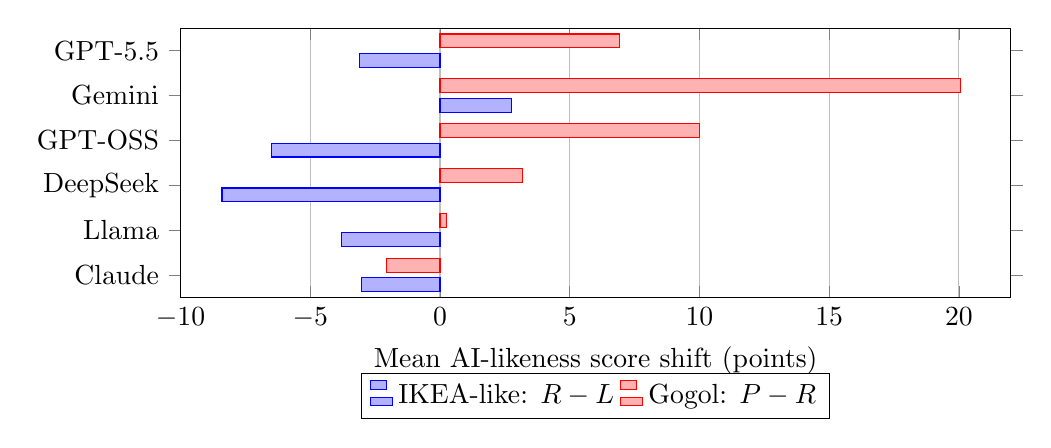
\begin{tikzpicture}
\begin{axis}[
    xbar, width=\linewidth, height=5.0cm,
    xmin=-10,xmax=22,
    symbolic y coords={Claude,Llama,DeepSeek,GPT-OSS,Gemini,GPT-5.5},
    ytick=data,
    xlabel={Mean AI-likeness score shift (points)},
    legend style={at={(0.5,-0.28)},anchor=north,legend columns=2},
    xmajorgrids=true,
    bar width=5pt]
\addplot coordinates {(-3.01,Claude) (-3.81,Llama) (-8.40,DeepSeek) (-6.48,GPT-OSS) (2.77,Gemini) (-3.10,GPT-5.5)};
\addplot coordinates {(-2.05,Claude) (0.24,Llama) (3.18,DeepSeek) (10.00,GPT-OSS) (20.06,Gemini) (6.91,GPT-5.5)};
\legend{IKEA-like: $R-L$,Gogol: $P-R$}
\end{axis}
\end{tikzpicture}
\caption{The writer-state-associated and completion-associated shifts differ qualitatively across models. Error bars and inferential details are reported in Appendix~\ref{app:adaptive}.}
\label{fig:decomp}
\end{figure}

\subsection{Level error and rank reliability are different failures}
Across the ten-model descriptive sweep, mean within-output LIVE--POST Spearman ranges from .329 to .820 while raw MAE ranges from 4.2 to 24.5 points. Claude Opus 5 and GPT-5.5 preserve local retrospective ordering well (mean $\rho=.820$ and $.817$), while Gemini and Qwen3 are much lower ($.345$ and $.329$). Yet Qwen has the smallest raw MAE (4.25), whereas Gemini has the largest (24.47). A model can therefore be close in absolute level while poor at local selection, or shifted in level while preserving ordering.

Five-fold grouped calibration reinforces the distinction. An affine mapping reduces held-out MAE for several models (e.g., Gemini from 24.47 to 20.43; GPT-OSS from 8.63 to 6.87), but any monotone affine correction leaves the within-output ranking unchanged. A controller that thresholds a score may benefit from recalibration; a controller that selects the worst span needs a separate rank audit. Full coverage and calibration tables appear in Appendix~\ref{app:coverage}.

\subsection{Held-out controls preserve the directional result}
A fresh 24-prompt extension repeated LIVE and POST under four semantically matched elicitation schemes for GPT-5.5 and Gemini. All eight model--elicitation mean $P-L$ shifts were positive with prompt-bootstrap 95\% intervals above zero. Averaged across variants within prompt, GPT-5.5 shifted $+5.33$ points and Gemini $+8.61$, with a matched difference of $+3.28$ (95\% CI $[0.72,5.97]$). On the pooled 40 robustness prompts, the matched Gemini-minus-GPT difference is $+4.57$ (95\% CI $[2.05,7.27]$). Rank reliability is more sensitive to the elicitation surface, which is itself an operational warning.

The temperature control addresses a concern that numeric score tokens sampled at $T=.7$ could create the apparent state shift. At $T=0$, GPT-5.5 has $R-L=-1.97$ and $P-R=+7.13$; Gemini has $R-L=-0.01$ and $P-R=+25.27$. Thus the positive post-completion component in these high-coverage models does not require stochastic score-token sampling. Temperature changes the generated prose trajectory too, so the $T=0$ versus $T=.7$ contrast is not a clean causal estimate of temperature itself.

\subsection{Good target ranking is not sufficient for one-shot correction}
The equal-compute rewrite check asks whether a useful LIVE ranking automatically translates into a useful correction policy. It does not. For GPT-5.5 ($N=40$), the guided advantage is $-0.28$ POST-score points; for Gemini, 37 valid pairs yield $+0.27$, with neither paired win-rate test significant. This null is particularly informative for GPT-5.5 because the LIVE target is retrospectively the highest-scored sentence in 72.5\% of outputs and in the top two in 87.5\%. Correctly locating a problematic span is not sufficient for this one-shot rewrite operator to improve the whole document. Gemini's much weaker LIVE--POST rank reliability also makes its granular POST delta a noisier outcome, so the GPT-5.5 null is the cleaner diagnostic. We do not generalize either result to stronger multi-turn self-correction methods.

\section{Discussion}
\paragraph{The original IKEA story is too simple.}
The motivating two-state pattern could be narrated as self-favoring while writing. REPLAY changes that conclusion. In five of six decomposed models, $R-L$ is negative, while four show positive $P-R$. Gemini can exhibit both: a small IKEA-like writer-state component followed by a much larger completion-associated component. GPT-OSS and DeepSeek V4 move in the opposite direction at REPLAY and then reverse after completion. A simple LIVE--POST difference hides these trajectories.

\paragraph{Why completion can matter.}
A later sentence can reveal repetition, formulaic structure, inconsistency, or a global pattern that changes how an earlier sentence looks. This is especially plausible for a holistic stylistic property such as AI-likeness. For locally verifiable mathematical or code steps, future context may matter less, and the decomposition may look different. The current results therefore motivate, rather than settle, generalization to objective reasoning.

\paragraph{Implications for inference-time control.}
The practical lesson is not that POST is superior. POST has information unavailable online. Instead, a controller should audit the property it actually consumes. Thresholding requires level stability or validated recalibration; local selection requires ordering stability; and any system comparing online and delayed scores should test whether later context creates a systematic state shift. A single scalar ``calibration'' summary can obscure these distinct failure modes.

\paragraph{Future work.}
Three extensions are especially important. First, open-weight models would permit stronger replay interventions that control token history and inspect hidden-state effects. Second, the protocol should be applied to objective endpoints---mathematical correctness, code execution, or process-verifier scores---where future-context dependence may differ from stylistic judgments. Third, live-score diagnostics should be integrated with stronger multi-turn correction policies to distinguish failure of target selection from failure of the correction operator.

\section{Limitations}
The endpoint is perceived AI-likeness of short social-writing outputs, not correctness. No human judgments enter the reported score endpoint, so the study establishes state-indexed consistency among model scores, not human-valid detection ability. REPLAY reconstructs visible text but cannot hold hidden activations, provider state, or prior score-token history fixed. Six models have sufficiently developed three-state data for the cross-model effect comparison, and four of those use adaptive breadth-extension sample sizes. Low protocol adherence for several other models can introduce survivorship bias in descriptive reliability comparisons. The robustness follow-up was frozen after an earlier cohort had been inspected, and the temperature control contains only 10 prompts. Hosted model routes can also change over time. These limitations bound the claim to a reproducible operational pattern in the tested model/serving configurations rather than a prevalence estimate over all LLMs.

\section{Conclusion}
A large discrepancy between online and retrospective self-scores need not be an IKEA-like ownership bias. In our six-model decomposition, only one model has a positive mean writer-state-associated shift, whereas four show positive post-completion self-devaluation. In the strongest case, roughly 88\% of the total retrospective shift appears only after the completed output is visible. We call this model-dependent pattern the Gogol effect. More generally, live self-scores should be treated as state-dependent control signals: their level, local ranking, and temporal stability require separate validation before they are used for search, selection, or self-correction.
